\chapter{太阳系中的物理过程}
\section{潮汐力}
如图\ref{fig:tidalforce} 由于地球本身尺度的原因,导致地球表面收到的月球引力不相等,产生差引力,这被称为\textbf{潮汐力}。地球上近月球端和远月端的潮汐力方向相反,这会使地球发生延地月连线方向的形变,引起涨潮现象,因此这种形变被称为\textbf{潮汐隆起}。

\begin{figure}[hbt]
  \centering
  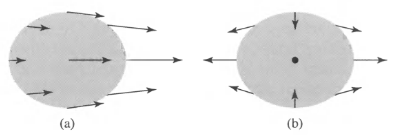
\includegraphics[width=10cm]{chapters/19/tidalforce}
  \caption{潮汐力示意图。(a)地球表面月球的引力(b)月球对地球的潮汐力(表面与地心的差引力)}
  \label{fig:tidalforce}
\end{figure}

为了理解潮汐力和潮汐隆起,尤其是背面的潮汐隆起,我们需要明白地球上每一点都受到月球的引力,近月段最强,中心较弱,远月端最弱。因此近月端的海水被拉像月球产生潮汐隆起,而远月端因为落后于被月球拉走的地球而产生隆起。两端的潮汐隆起导致了我们一天能看到两次涨潮。

通过计算,我们可以得到引力随距离的大小变化为:
\begin{equation}
  dF_m=-2G{Mm\over r^3}\;dr
\end{equation}

对于地球来说,可以得到潮汐力为:
\begin{equation}
  \Delta F\simeq{GMmR\over r^3}\left(2\cos\theta\,\hat{\mathbf i}-\sin\theta\,\hat{\mathbf j}\right)
\end{equation}

其中$R$是地球半径,$r$是地球中心到月球的距离,$\theta$是地球表面一点与地月方向的夹角,而在地月连线上$\Delta F=-2G{Mm\over r^2}$。从式中可以发现,两个天体距离越近的时候,潮汐力越显著。

\begin{figure}[hbt]
  \centering
  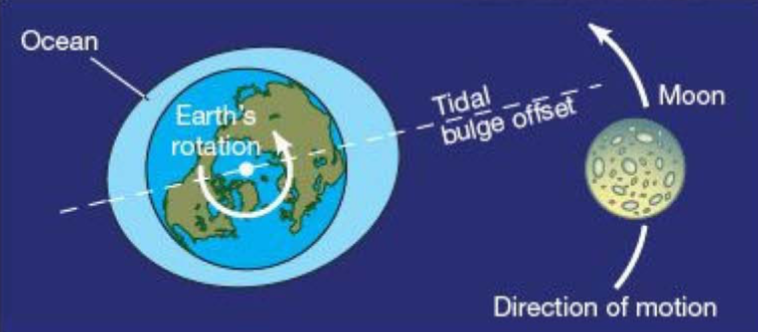
\includegraphics[width=10cm]{chapters/19/tidalbulge}
  \caption{地球自转引起潮汐隆起不准确指向月球}
  \label{fig:tidalbulge}
\end{figure}

潮汐力的另一个作用是会使地球的自转变慢。如图\ref{fig:tidalbulge},由于地球的自转比公转快,地壳与海洋以及地球内部的摩擦效应会使潮汐隆起会有被拖动着与地球一起转的趋势,这导致了隆起部分并不严格指向月球,而这种长期的摩擦会导致地球的自转变慢,最终与公转周期相同,这种效应被称为\textbf{潮汐锁定}。月球就是一个已经被地球的潮汐力锁定的天体,因此月球永远是固定的一面朝着我们。

\subsection{洛希极限}
那么我们可以想象,当潮汐力足够大的时候,天体甚至能够被撕裂,这种现象常常发生在黑洞这类的致密星附近。要撕裂一个天体,潮汐力需要克服引力,前面算出,距离越近,潮汐力越强,洛希在1850年计算得到了这个临界距离,此后被称为\textbf{洛希极限}:
\begin{equation}
  r<f_R\left(\bar \rho_P \over \bar \rho m\right)^{1/3}R_p
\end{equation}

其中$f_R=2.456$。

\section{大气的物理}
\subsection{大气温度}
行星的温度来源于太阳的辐射,因此我们可以考虑行星的反照率为$a$,即吸收了(1-$a$)倍的辐射升温,同时行星还会以黑体辐射的方式辐射热量,假设到太阳的距离为$D$,我们可以计算出热平衡下行星大气的温度为:
\begin{equation}
  T_p=T_\odot(1-a)^{1/4}\sqrt{R_\odot \over 2D}
\end{equation}

\subsection{大气成分}
由于行星的大气之外是真空,时刻在做无规则热运动的气体分子受行星引力束缚在行星表面,但温度越高,气体分子运动越剧烈,就越有可能逃离行星。

根据麦克斯韦-玻尔兹曼速率分布和行星表面的逃逸速度,我们可以计算得到分子的逃逸温度:
\begin{equation}
  T_\mathrm{esc}>{1\over54}{GM_p m \over kR_p}
\end{equation}

其中$m$是气体粒子的质量。通过上式可以知道,质量越大的粒子可以在较高温度的大气中存在,较轻的粒子则会逃离行星表面。结合前面计算得到的行星大气温度,我们可以知道行星大气中可能存在的气体成分。
